\section{Actors and Roles}
The TrainingMS system defines three distinct user profiles to ensure secure and efficient operations:
\begin{itemize}
    \item \textbf{Simple User}: An operational user responsible for the daily management of training data. Their functionalities include authentication (login/logout), management of formations (creation, editing, deletion, and viewing), participants, and trainers. They also handle assignments, such as enrolling participants and associating trainers with specific sessions.
    \item \textbf{Manager (Responsable)}: An analytical user focused on evaluation and decision-making. Unlike the Simple User, the Manager has **read-only access** to the system's core data and cannot perform any modification, creation, or deletion. Their primary focus is the statistics dashboard, where they analyze formation counts, participant data, and budget distribution through interactive charts and advanced filters.
    \item \textbf{Administrator}: A high-level actor with full control over system configuration. Administrators manage user accounts and core referential data (domains, structures, profiles). By inheritance, the Administrator has access to all functionalities of **both** the Simple User (for data management) and the Manager (for analytical overview).
\end{itemize}

\section{Functional Requirements}
The application must support the following core capabilities:
\begin{itemize}
    \item \textbf{Authentication}: Secure login and logout using JSON Web Tokens (JWT).
    \item \textbf{CRUD Operations}: Comprehensive management (Create, Read, Update, Delete) for participants, trainers, sessions, and reference tables.
    \item \textbf{Training Planning}: Ability to schedule sessions, assign trainers, and enroll participants.
    \item \textbf{Dashboarding}: Real-time display of aggregated statistics and trends.
\end{itemize}

\section{Non-Functional Requirements}
To ensure a professional-grade application, several non-functional aspects were prioritized:
\begin{itemize}
    \item \textbf{Security}: Implementation of role-based access control (RBAC) and password encryption.
    \item \textbf{Performance}: Optimization of database queries to handle growing datasets efficiently.
    \item \textbf{Usability}: A responsive and intuitive user interface designed to minimize the learning curve.
    \item \textbf{Data Integrity}: Strict adherence to relational constraints and input validation.
\end{itemize}

\section{UML Design}
\subsection{Use Case Diagram}
The Use Case Diagram illustrates the interactions between the identified actors and the system's functionalities. The primary use cases include "Manage Formations", "Register Participants", and "Consult Dashboard", with administrative tasks such as "Manage Users" reserved for the Admin actor.

\begin{figure}[H]
    \centering
    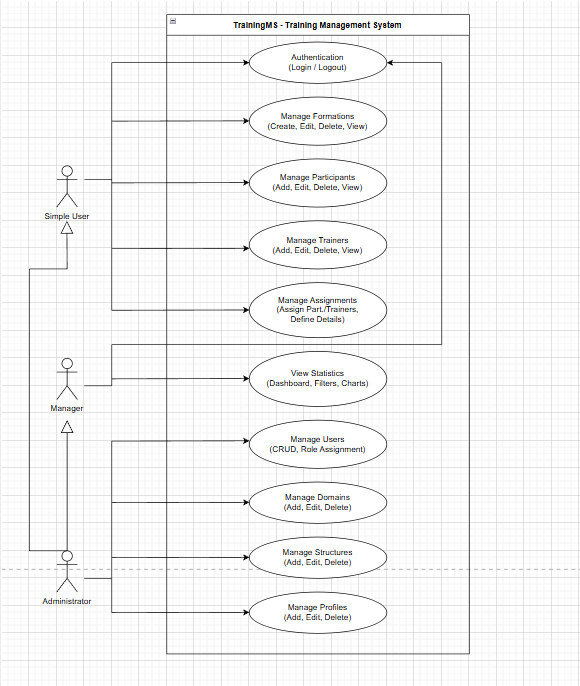
\includegraphics[width=0.8\textwidth]{Figures/Use case diagram.png}
    \caption{TrainingMS Use Case Diagram}
    \label{fig_use_case}
\end{figure}

\subsection{Class Diagram}
The core logic of the system is modeled through several interrelated entities:
\begin{itemize}
    \item \textbf{User \& Role}: Manage security and permissions.
    \item \textbf{Training Session}: The central entity representing a training session.
    \item \textbf{Participant \& Trainer}: Entities representing the human capital involved.
    \item \textbf{Domain, Structure, Profile}: Referential entities that categorize the data.
\end{itemize}
Relationships include a Many-to-Many association between \textit{Training Session} and \textit{Participant} (registrations) and Many-to-One links from \textit{Training Session} to \textit{Domain} and \textit{Trainer}.

\section{Database Design}
The relational schema was designed in MySQL to ensure optimal storage and fast retrieval. The database includes:
\begin{itemize}
    \item \textbf{Tables with Primary Keys}: All tables use auto-incremented integers as unique identifiers.
    \item \textbf{Foreign Key Constraints}: Relationships are enforced through foreign keys (e.g., \textit{idDomain} in the \textit{training session} table).
    \item \textbf{Integrity Rules}: Cascade operations and nullability constraints are defined to prevent orphaned records.
\end{itemize}
This structured approach guarantees that the data remains consistent throughout the application's lifecycle.
